% LaTeX Template for short student reports.
% Citations should be in bibtex format and go in references.bib
\documentclass[a4paper, 11pt]{article}
\usepackage[top=3cm, bottom=3cm, left = 2cm, right = 2cm]{geometry} 
\geometry{a4paper} 
\usepackage[utf8]{inputenc}
\usepackage{textcomp}
\usepackage{graphicx} 
\usepackage{amsmath,amssymb}  
\usepackage{bm}  
\usepackage[pdftex,bookmarks,colorlinks,breaklinks]{hyperref}  
\hypersetup{linkcolor=black,citecolor=black,filecolor=black,urlcolor=black} % black links, for printed output
\usepackage{memhfixc} 
\usepackage{pdfsync}
\usepackage{fancyhdr}
\pagestyle{fancy}

\title{\Huge{Autonomous Software Agents} \\ \Large{Project Report} \\ \footnotesize{AGVZZ Group}}

\author{
\begin{tabular}{cc}
\parbox{7cm}{\centering Francesco Vaccari [239927] \\ \small{\centering francesco.vaccari@studenti.unitn.it}} & 
\parbox{7cm}{\centering Simone Compri [239953] \\ \small{\centering simone.compri@studenti.unitn.it}}
\end{tabular}
}

\date{}

\begin{document}
\maketitle
\tableofcontents


\pagebreak

\section{Implementation of BDI}

The objective of this project consists of developing autonomous software agents, namely a single operating agent and a pair of cooperating agents, for the Deliveroo.js game.
To accomplish it we created software agents based on the BDI architecture in order to make it possible for them to analyze the environment and act accordingly.\\
More precisely, an agent can perceive the environment and organize that information categorizing it into different classes and creating a set of \textbf{Beliefs} (i.e., \emph{Environment properties}, \emph{Game Map}, \emph{Parcels}, the \emph{Agent} itself, the \emph{Allied Agent}, \emph{Enemy Agents}, \emph{Joint Parcels Set} and \emph{Joint Agents Set}).\\
After that, that information is analyzed relying on some \textbf{Intention Rules} that are filtered in such a way to obtain a series of targets, categorized by coordinates, an \textbf{Intention} between \emph{idle}, \emph{pickup}, \emph{delivery}, \emph{exchange} and \emph{block} and a score.\\
Once deliberated the target with the best score, it is took as argument by a \textbf{Planner} which computes a \textbf{Plan} composed by the series of actions (i.e. \emph{up}, \emph{down}, \emph{left}, \emph{right}, \emph{pickup} or \emph{putdown}) that the agent will perform.\\
If it fails, the intentions will change as a consequence and a new \textbf{Plan} will be computed. In fact, in the meanwhile the environment can change, so, a \textbf{Revision} of \textbf{Beliefs}, \textbf{Intentions} and \textbf{Plans} that fail is done when it happens.\\
\\

\begin{figure}[h]
    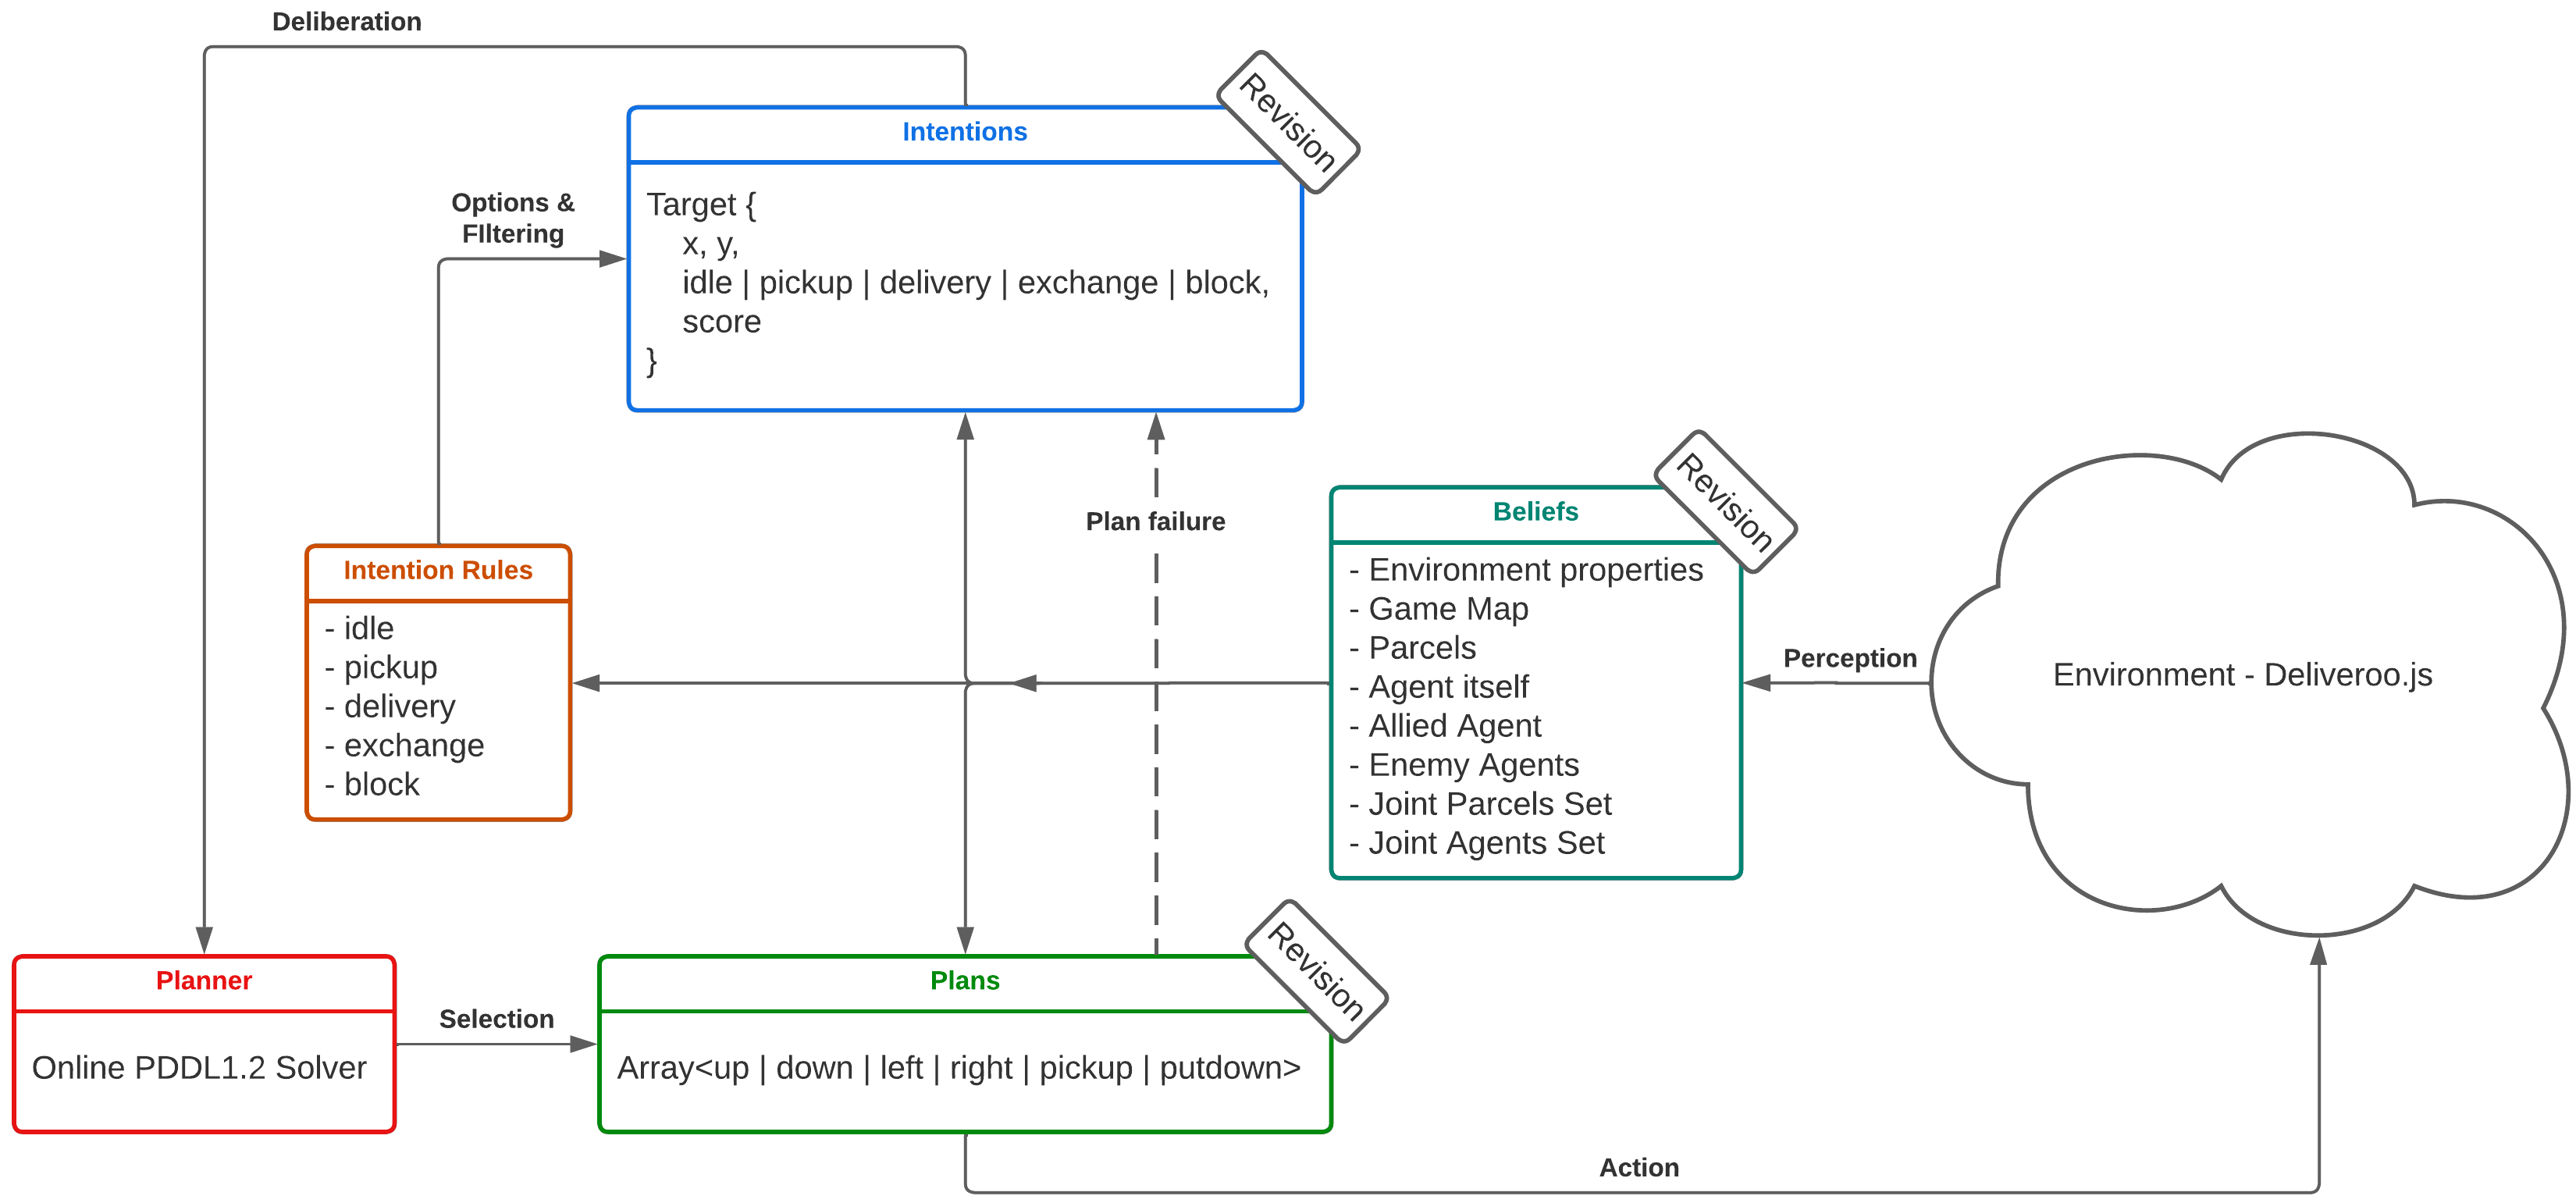
\includegraphics[width=\textwidth]{images/BDI schema.png}
    \caption{BDI schema}
    \centering
\end{figure}

\pagebreak


\section{Single-Agent Architecture}


\subsection{Beliefs Sets and Beliefs Revision}
Most of the belief sets implemented can be considered knowledge, facts that the agent knows certainly are true. Only with regard to parcels and agents, some information that might not be true is stored; this allows the agent to have some memory which is fundamental for planning. The belief sets implemented reflect all the variable elements of the environment:
\begin{itemize}
\item \textbf{Environment properties}: After connection of the agent, 3 important variables are set: parcels and agents viewing distances and the parcels decaying interval (if present). These values are used to implement visibility and decay of parcels and visibility of enemy agents.
\item \textbf{The Agent Itself}: Each time the listener \verb|onYou| is called, score and coordinates of the agent are updated.
\item \textbf{Game Map}: After connection to the server, through \verb|onMap|, the agent receives  information about the cells that constitute the game map. Each cell is initialized and then stored into a matrix to use later during planning. The attributes of the cells describe their position in the map and whether they are deliverable cells, spawning cells, normale walkable cells or walls. Furthermore, each cell is initialized with an attribute \verb|lastSeen| that counts how much time has passed since the agent has last seen the cell; this value is necessary to implement and plan the idle searching movement.
\item \textbf{Parcels}: Each parcel is identified by an id and described by its position in the map, reward and whether it is currently being carried. Along with these values, we added a visibility attribute. This lets us keep track of parcels that are not currently within the viewing area of the agent to improve planning capabilities. Also, the decaying interval is used to update parcels that are not visible by the agent. Knowing the agent's viewing distance is useful also to correct inconsistencies in the parcels stored; for example, when an enemy agent picks up a parcel that is not currently visible, the agent will not know that the parcel is not there anymore until the old coordinates are seen by the agent. The revision of this belief set happens whenever \verb|onParcelsSensing| is called.
\item \textbf{Agents}: Similarly to parcels, each agent is identified by an id, and is described by its position, score and visibility. These values get updated whenever \verb|onAgentsSensing| is called. The visibility attribute is computed by knowing how far away our agent can see enemies. An agent that is not visible for more than three seconds is deleted by the belief set, this allows us to remember the position of enemies in the recent past without really impacting future decisions since it's very likely that after that amount of time the last known position is no longer accurate.
\end{itemize}

As explained, the beliefs revision process happens asynchronously with respect to the computation and execution of the plan. This allows the agent to always have at hand the most recent and consistent information about itself and about the various elements of the environment.

\subsection{Intentions and Intentions Revision}
For the single-agent architecture we identified 3 possible intentions:
\begin{itemize}
\item \textbf{Search for parcels}: This is the behavior which can be considered as default, and it is chosen when the agent is not carrying any parcel and does not know the position of any parcel. This intention is also chosen when the plan to perform any other intention would fail if executed: for example, when an enemy agent is blocking the only path that leads to the only parcel in view. In the code, this intention is identified as \verb|idle|, and is implemented using a \verb|lastSeen| attribute assigned to each cell in the map. This attribute indicates how much time has passed since the last time the agent saw that specific cell. When the agent chooses this intention, it travels around the map picking as target the cell with the highest \verb|lastSeen| value; and since this value is update asynchronously, as soon as the agents sees that the cell is empty, the attribute is updated and the target of this intention is changed.
\item \textbf{Pickup a parcel}: When the parcels belief set is not empty, if the agent decides to pick up a parcel, the intention chosen is \verb|pickup|. When this happens the parcel is picked as target and the agent starts moving towards the correct cell.
\item \textbf{Deliver parcels carried}: When the agent is carrying parcels, if it is deemed the best decision, the agent will choose to perform the \verb|delivery|. The target of this intention is the closest delivery cell that can be reached from the agent's position.
\end{itemize}

\subsubsection{Utility Functions}
The way the intentions are implemented is complex to handle situations in which the agent has to decide if it should deliver the parcels it is carrying or if it should change its intention to go pick up more parcels in its viewing distance. Furthermore, since there might be agents that are trying to accomplish the same ultimate goal of scoring more points, the agent has to consider enemies distances to certain cells. Modeling the wanted behavior in such situations can be really challenging, and so we decided to implement a system which assigns to each cell in the map a score. These scores are asynchronously recomputed and the cell with the highest value is chosen as the target. The score is the output of an utility function which takes as input all the elements in the environment and outputs a score map using two formulas we designed: one for cells with the property of spawning parcels, and one for cells assigned as delivery.

Next is the formula used to compute the score for a spawning or normal cell with coordinates $x,y$:
\begin{equation}
score(x,y) = \left(\frac{{ParcelsRewardInCell(x,y)^{1.2}}}{{DistanceToAgent(x,y)}}\right) \cdot EnemyProximity(x,y,agents)^2
\end{equation}
In the formula, $ParcelsRewardInCell$ is the sum of the rewards of the parcels in the cell, while $DistanceToAgent$ is the minimum path length to the agent. $EnemyProximity$ is computed as follows:
\begin{equation}
EnemyProximity(x,y,agents) = -(\frac{1}{\min_{a_{i} \in \{agents\}} Distance(x, y, a_{i}.x, a_{i}.y) +1}) + 1
\end{equation}
The $Distance$ function used is the Manhattan Distance. As default, when no enemy agents are known, the value of $EnemyProximity$ is set to $1$. Otherwise, the formula outputs a value in the range $[0,1]$ that acts as a scaling factor that discourages the agent to choose parcels, even with high reward, when they are very close to enemy agents.

Below there is the formula used for cells assigned for delivery:
\begin{equation}
\frac{ParcelsRewardsCarried^{~0.8}}{DistanceToAgent(x,y)}
\end{equation}
The term $ParcelsRewardsCarried$ indicates the sum of the rewards of the parcels carried by the agent while $DistanceToAgent$ is the minimum path length from the agent to the cell.

Considering all the elements in the environment and combining them with distances between elements and different rewards of the parcels results in a behavior that is reactive and adapts to the frequent changes on the map. This process of computing scores is continuous and asynchronous and allows for an easy decision of the intention to choose. Since each score is related to a cell, the coordinates of the target are ready as soon as the highest score is found so that the plan can be immediately calculated. This makes it also possible to have backup targets since they are sorted in a list, this is useful in case the planner does not find a path for the first candidate target.

\subsection{Planning}

This task is implemented in the class \verb|Planner| and takes as input all the elements of the beliefs sets (map, agents and parcels list and the current agent) and, after the intentions are computed, it creates the plan that the agent is going to use.
More precisely, the task that the solver has to solve consists of a BFS (Breadth-First Search) that:
\begin{itemize}
    \item Is performed on the game map, considered as an undirected graph, where the cells are the nodes and the proximity to other cells define the edges;
    \item Uses the agent position as root;
    \item Ends when the shortest path to the target cell is found.
\end{itemize}

Tho compute the plan, the planner relies on an online solver for PDDL1.2 (Planning Domain Definition Language) As the standard declares, the model of the planning problem is composed by two major parts:
\begin{enumerate}
    \item Domain description: defines the predicates that characterize the environment and the action that can be performed.
    \item Problem description: describe objects in the environment, the initial state and goal descriptions that will characterize the current plan.
\end{enumerate}

\subsubsection{Domain Description}

Since the tasks consists of a BFS, the domain file models the environment, composed by cells and the agent, into an undirected graph.
More precisely, the domain is composed of:
\begin{itemize}
    \item Predicates:
    \begin{itemize}
        \item \emph{cell ?x\_y}: it indicates that the object \emph{x\_y} is a cell and a node of our graph
        \item \emph{near ?from\_x\_y ?to\_x\_y}: it models that the cell \emph{from\_x\_y} is near the cell \emph{to\_x\_y}, i.e., there is a unidirectional edge from the first to the second (in the Problem description section it is explained how the graph becomes undirected)
        \item \emph{in ?x\_y}: it keeps track that the agent is in the cell \emph{x\_y}. In the graph parallelism it refers to the node that the planner is visiting
    \end{itemize}
    \item Actions:
    \begin{itemize}
        \item \emph{move}: it represents the agent movement through the map (i.e, the graph). It takes as parameters two objects \emph{from\_x\_y} and \emph{to\_x\_y}, which respectively represent the starting and the target cell of the movement. Then it checks if the agent is in \emph{from\_x\_y} (i.e., \emph{from\_x\_y}), if the object \emph{to\_x\_y} is a cell (i.e., \emph{cell to\_x\_y}) and if the two cells \emph{from\_x\_y} and \emph{to\_x\_y} are close (i.e., \emph{near from\_x\_y to\_x\_y}).
        After that, the effect of the action consists in moving the agent to the target cell (i.e., \emph{in to\_x\_y}) and making sure that it is different from the starting cell (i.e., \emph{not (in from\_x\_y}).
    \end{itemize}
\end{itemize}

In the move action we avoid to put the precondition \emph{cell from\_x\_y} because we assume that the starting point of the plan taken from the intentions is a cell. After that, thanks to the combination of the precondition \emph{cell to\_x\_y} and the effect \emph{in to\_x\_y} we know that all the following objects are cells.

Here is the domain description just described:
\begin{verbatim}
    (define (domain deliveroo)
        (:requirements :strips)
        (:predicates
            (cell ?x_y)
            (near ?x_y ?x_y)
            (in ?x_y)
        )
        
        (:action move
            :parameters (?from_x_y ?to_x_y)
            :precondition (and (in ?from_x_y) (cell ?to_x_y) (near ?from_x_y ?to_x_y))
            :effect (and (in ?to_x_y) (not (in ?from_x_y)))
        )
    )
\end{verbatim}

\subsubsection{Problem description}

The problem description is created in two different phases.
First of all, when the map is initialized, we visit the matrix and for each cell that isn't a wall we identify it as \emph{c\_x\_y}, where \emph{x} and \emph{y} are its coordinates, and declare (i.e., add the proper objects and put the proper predicate in the \emph{init} section) that it is a cell (i.e., \emph{cell c\_x\_y}) and, for every neighboring cell (identified with the same notation) that is not a wall, we sign that they are close (i.e., \emph{near c\_x\_y c\_\(x_1\)\_\(y_1\)}).\\
Then, when we have to compute a plan, we look at in which cells \emph{c\_x\_y} the other agents are in and we treat each of them as walls (i.e., \emph{(not (cell c\_x\_y))}). After that, we declare in which cell \emph{c\_x\_y} the agent is (i.e., \emph{in c\_x\_y}) and we set the target cell \emph{c\_\(x_1\)\_\(y_1\)}, taken from the intentions as the goal of the plan (i.e., \emph{in c\_\(x_1\)\_\(y_1\)}).\\
These two actions are performed always taking the problem description of the map described before and updating it at the current situation as just described.

\subsubsection{Implementation}

The planner is executed as many times as possible. In fact, there are "threads" of the program that set up the targets and, when the agent is waiting still, the procedure \emph{pddlBFS} is called and the respective plans are computed.\\

After the planner has computed the plan, we translate it in the language that the agent can understand. In fact, we parse the coordinates contained into the objects \emph{from\_x\_y} and \emph{to\_x\_y} and compute if the movement corresponds to \emph{up}, \emph{down}, \emph{left} or \emph{right}. After that we append to the plan the intention \emph{pickup} or \emph{putdown} computed before.\\

\subsubsection{PDDL example}

Consider this situation of the map: [0 wall, 1 free cell, 4 agent]
\begin{verbatim}
    [
        0 ->
        | [1, 1, 1, 1],
        v [0, 4, 1, 0],
          [1, 1, 1, 1],
          [1, 0, 0, 0]
    ]
\end{verbatim}

The problem description created is as follows:
\begin{verbatim}
    (define (problem BFS)
        (:domain deliveroo)
        (:objects c_0_0 c_0_1 c_0_2 c_0_3 c_1_1 c_1_2 c_2_0 c_2_1 c_2_2 c_2_3 c_3_0)
        (:init 
            (cell c_0_0) (cell c_0_1) (cell c_0_2) (cell c_0_3)
            (not (cell c_1_1)) (cell c_1_2)
            (cell c_2_0) (cell c_2_1) (cell c_2_2) (cell c_2_3)
            (cell c_3_0)
            (near c_0_0 c_0_1)
            (near c_0_1 c_0_0) (near c_0_1 c_1_1) (near c_0_1 c_0_2)
            (near c_0_2 c_0_1) (near c_0_2 c_1_2) (near c_0_2 c_0_3)
            (near c_0_3 c_0_2)
            (near c_1_1 c_0_1) (near c_1_1 c_2_1) (near c_1_1 c_1_2)
            (near c_1_2 c_0_2) (near c_1_2 c_1_1) (near c_1_2 c_2_2)
            (near c_2_0 c_3_0) (near c_2_0 c_2_1)
            (near c_2_1 c_1_1) (near c_2_1 c_2_0) (near c_2_1 c_2_2)
            (near c_2_2 c_1_2) (near c_2_2 c_2_1) (near c_2_2 c_2_3)
            (near c_2_3 c_2_2)
            (near c_3_0 c_2_0)
            (in c_0_3))
        (:goal (in c_3_0))
    )
\end{verbatim}

And the plan that is created is:
\begin{verbatim}
    (move c_0_3 c_0_2) -> down
    (move c_0_2 c_1_2) -> right
    (move c_1_2 c_2_2) -> right
    (move c_2_2 c_2_1) -> down
    (move c_2_1 c_2_0) -> down
    (move c_2_0 c_3_0) -> right
\end{verbatim}

\subsubsection{Considerations}

The choice to assign to the planner "only" the BFS task relies on two factors.
\begin{itemize}
    \item The first one is regarding the complexity of PDDL solver. In fact, since it is exponential in the number of actions and polynomial in the number of states, reducing the number of actions to only one (the move action) means reduce the overall complexity. In this way the latency is considerably reduced, since the major complexity of the solver is simplified, and the remaining latency is the sum of the one given by the polyomial part of the solver algorithm and the one of the network.
    \item The second one takes into consideration how the PDDL planner works. Indeed, considering that starting from the starting cell (initial state) and moving through the nearby cells (action move) until it reaches the target cell (goal), the first plan found (i.e, the shortest) coincides with the shortest path bewteen the starting and the target cell
\end{itemize}

\subsubsection{Offline version}

Since the online solver adds a latency due to the network latency we created an offline version of the BFS method that works completely synchronously with the code and reduces considerably the time taken by the planner to compute the plan.

%\pagebreak

\section{Multi-Agent Architecture}

\subsection{Communication}
\subsubsection{Initialization}
In order to allow the two agents to exchange information about intents and beliefs, a communication needs to be established in the first few moments of the execution of the programs. A simple protocol, composed of 3 types of messages, allows the agents to recognize each other and discover the agent ids that will be used after the initialization is completed successfully.

The agents are assigned two different roles: sender and receiver. The sender forwards the first INIT message while the other agent waits to receive the request of initialization. After the request is received, a SECRET message is sent back in order to confirm the identity to the first agent which will respond with an OKAY message that will end successfully this first phase of communication. After these 3 messages are exchanged, both agents know the id of each other; this id will be used in all future exchanges of information.

\subsubsection{Handling of messages}
Once the communication is initialized, each agent will start sharing the information about its beliefs sets and intentions. A buffer is used to store temporarily the messages waiting to be processed by a function that modifies variables or information stored according to the type of the message received. The implementation of the handler affects the following information kept by the agents:
\begin{itemize}
\item \textbf{Friend Agent}: Each agent sends constantly its updated position, score, total reward of parcels carried and current target of the plan in execution. This allows better decisions while choosing for targets and avoids the generation of conflicting plans.
\item \textbf{Enemy Agents}: Since each agent has its own list of enemies that it sees, when this list is updated a message is sent so that the other agent can utilize the information during planning.
\item \textbf{Parcels}: When the belief set regarding parcels is updated, a message is sent in order to let the other agent know the most recent confirmed state of visible parcels.
\item \textbf{Map}: The handling of this type of messages has the sole purpose of provide better information for the idle searching movement implemented in the planner. Each time an agent moves it sends information about the cells that are visible so that both agent's maps are consistent with each other.
\item \textbf{Exchange Intention}: Whenever the planner decides to perform the exchange of parcels there is the need to communicate the intention to the other agent and to also update internal planning targets whenever they are not computed locally. Moreover, there is the need to handle the exit from the intention exchange whenever an error occurs or the process ends successfully.
\item \textbf{Block Strategy Intention}: Similarly to the exchange intention, there is also the need to handle messages that allow the agents to coordinate when a planner decides to perform the blocking strategy.
\end{itemize}

\subsection{Beliefs and Beliefs Revision}
In addition to the belief sets of the single-agent architecture, some more sets were added to enable the implementation of more complex behavior and allow the coordination between the agents. Below is the list of the new beliefs added:
\begin{itemize}
\item \textbf{Joint Parcels Set}: We decided that the best and easiest way to implement a joint belief set was to let each agent have its own set that is sent via message when updated, and then the message handler has the duty to build the joint set. Only the complete set is used while planning. This allows us to reuse the implementation of the beliefs set of the single-agent architecture and to only build on top of it. The sharing of parcels positions and visibilities makes it less likely that an agent is left searching for targets to pickup.
\item \textbf{Joint Agents Set}: The same design decision has been implemented for the agents beliefs set: the two different sets get synced up when an update is received.
\item \textbf{Enemy Agents}: This belief set was implemented specifically to enable a particular intention that will be explainer later: the blocking strategy. This internal representation of enemies stores the information regarding up to two agents that are competing with our cooperating duo. The information stored consists of ids, scores, positions and visibilities, and is shared between our agents.
\item \textbf{Ally Agent Representation}: This information is crucial to the implementation of multi-agent plans because it allows only one agent to perform all the computation necessary. The information stored is not limited to coordinates and score, but extends to details about the current target and the total reward of parcels that are being carried.
\end{itemize}

Just like for the single-agent architecture, updates of each set happen asynchronously and are triggered by the events \verb|onYou|, \verb|onParcelsSensing| and \verb|onAgentsSensing|.


\subsection{Intentions and Intentions Revision}
The default behavior of both agents, where no coordination is needed, is the same of the single-agent architecture. The utility functions put in place are the same with the only exception of an if statement added in the score evaluation of cells: if a cell is already the target of the other agent, its score is set to zero. This simple feature avoids conflicts that can happen when, for example, both agents choose the same parcel to pick up. Everything else we explained for the single-agent architecture remains valid for this part, with the only difference that since the information about the environment is shared, the effectiveness of the utility functions is improved.

In the multi-agent architecture we identified two major possible multi-agent intentions, called in the code with the terms \verb|exchange| and \verb|block|.
\begin{itemize}
\item \textbf{Exchange}: This intention allows the agent requesting an exchange to leave the parcels on the ground so that the other agent can pick them up. This intention is necessary when only one path to a delivery cell is possible for both agents, in this case the single-agent behavior would cause the agents to become obstacles for each other on the map. This intention is chosen only when an agent sees that in its path to a delivery cell there is the other agent to which it can request the exchange. We implemented an utility function that allows the agent that receives the request of exchange to temporarily ignore the request and finish delivering the parcels carried first. In this case, the agent requesting the exchange will move towards the other agent until it terminates its own intention. Instead, if the request is immediately accepted, both agents move towards each other and perform the exchange when at one cell of distance. All the computation is done only by the agent requesting the exchange to simplify the task of coordination, while the second agent sets its target with the messages it receives by the first agent.
\item \textbf{Block}: This strategy consists of physically blocking the only delivery cells on the map to not allow enemies to score any more points, and thus resulting in an automatic win. This intention is triggered when the information stored in the beliefs sets satisfy four conditions:
\begin{itemize}
\item The map has only 2 delivery cells and both are reachable for our agents;
\item Our total score is greater that the opponent's total score;
\item We see both enemy agents, this allows to have certain information about score and position on the map;
\item The path to both delivery cells for our agents is shorter than the path of enemy agents.
\end{itemize}
When these four conditions are together satisfied each agent picks the closest delivery cell as the target. This should result in a situation in which no team is able to deliver any cell. The computation and the checks for satisfiability of the conditions are carried on by one agent only to simplify coordination.
\end{itemize}

 
\subsection{Planning}

In this multi-agent version the PDDL planning strategy is basically the same as the single-agent one. The parts that have been changed rely on the fact that now the agent has also to interact with another ally. More precisely, after a communication with the other allied agent and based on the intention and the target, now the planner has to create also plans designed to make exchanges of parcels and blocking strategies to avoid that the enemies gain more points. This is done through various combination of the PDDL BFS used in the single-agent version.\\
Moreover, because of the increase in code complexity due to the increase in intentions to be handled, the planner now isn't called as much as possible, but only when the target (so the intentions) changes or after a certain amount of time.

%\bibliographystyle{abbrv}
% \bibliography{references}  % need to put bibtex references in references.bib
\end{document}